\chapter{Auswertung vorhandener Anwendungen}

Um eine fundierte Grundlage für die Entwicklung einer allgemein akzeptierten Hochschul-\ac{App} zu schaffen, muss erst analysiert werden, welche Alternativen die Hochschule Hof bereits anbietet und wie zufrieden die Nutzer dieser Anwendungen mit ihnen sind. Im folgenden wird demnach erst eine Zufriedenheitsumfrage untersucht, worauf die vorhandenen Anwendungen analysiert werden, bei denen dann gezielt auf die in der Umfrage gefundenen Mängelpunkte geachtet werden kann.

\section{Allgemeine Auswertung der Zufriedenheit\label{sec:umfrage}}

Im Rahmen der Analyse der vorhandenen Anwendungen der Hochschule Hof wurde eine Befragung der Studierenden durchgeführt. Diese richtete sich an zwei verschiedene Nutzergruppen und wurde demnach ebenfalls in zwei unterschiedlichen Fassungen durchgeführt, welche später genauer beleuchtet werden. Das Ziel dieser Umfrage ist die Erfassung des allgemeinen Zufriedenheitsstands der Nutzergruppen mit dem aktuellen Angebot an Anwendungen der Hochschule Hof, welche den Studenten Stundenplaninformationen und möglicherweise noch weiteres liefern.

\subsection{Zielgruppen}
\label{umfrage_zielgruppen}

Die Befragung der Studierenden richtet sich an zwei Benutzergruppen der aktuellen Stundenplananwendungen der Hochschule Hof. 
%Deutsche
Die deutlich größere der beiden Nutzergruppen, auf die auch das Hauptaugenmerk in der Entwicklungsphase der neuen Hochschul-\ac{App} liegt, sind die deutschsprachigen Studierenden der Hochschule Hof, welche dauerhaft als Studenten eingetragen sind. Diese Teilnehmergruppe der Umfrage besteht aus 225 anonymen Studierenden. 
%Prozentsatz von allen?
Diese Nutzergruppe stellt den Regelfall der Nutzung der \ac{App} dar. Die Studierenden sind alle immatrikuliert, belegen genau einen Studiengang und sind in einer Fakultät eingeschrieben. Der Regelstudent hat somit in den Grundlagen- und Kernbereichen seines Studiums einen festen Stundenplan, welcher sich nach dem Fachsemester dessen richtet. Dies macht die Entwicklung einer verbesserten Hochschul-\ac{App} deutlich einfacher, da viele Faktoren vorgegeben sind und kaum Spezialfälle abgedeckt werden müssen. Mögliche Abweichungen sind hier lediglich Langzeitstudierende und Zwischensemester.
\\
\linebreak
%Internationals
Die kleinere der beiden befragten Nutzergruppen bilden die internationalen Studierenden der Hochschule Hof, welche sehr wahrscheinlich eine andere Sprache als Deutsch als Muttersprache nutzen und nur zeitlich begrenzt an der Hochschule Hof eingeschrieben sind. Die Gruppe der Befragten umfasst 31 anonyme Studierende. 
%Prozentsatz von allen?
Diese Studierenden kommen oft aus Hochschulen, deren Organisation sich von der der Hochschule Hof deutlich unterscheidet. Somit ist eine Aufteilung dieser Nutzer in die drei Fakultäten der Hochschule deutlich schwieriger. Auch die Auswahl der Vorlesungen aus den Studiengängen unterscheidet sich in der Regel vom beschriebenen Normalfall, somit belegen viele Studierende aus dem Ausland oder aus anderen Hochschulen oft Vorlesungen aus verschiedenen Fakultäten und unterschiedlichen Studiengängen und Fachsemestern. Dies macht die Erstellung von passenden Stundenplänen für die betroffenen Internationalen deutlich komplexer und bedarf deshalb eine genaue Betrachtung der Zufriedenheit dieser Studierenden mit dem aktuellen Angebot an Anwendungen der Hochschule Hof, um deren Bedürfnisse besser zu erkennen.

\subsection{Ergebnisse\label{sec:umfrage_erg}}

%Allgemein
Aus den Befragungen ergab sich, dass 92\% der regulären Studierenden eine der drei Smartphone Anwendungen der Hochschule nutzen. Bei den internationalen Teilnehmern lag diese Zahl lediglich bei etwa 74\%. Die Nutzungshäufigkeit der Anwendungen ergab bei beiden Gruppen, dass mehr als drei viertel der Befragten die \ac{App} mindestens zwei bis drei mal wöchentlich nutzen. Aus den Antworten der internationalen Studierenden der Hochschule Hof ergibt sich ebenfalls, dass nur etwa 61\% alle studienrelevanten Informationen aus den Anwendungen der Hochschule beziehen können. Zudem sagen nur etwa 29\%, dass es ihnen leicht fällt, einen vollständigen Stundenplan zu erstellen. Diese Erkenntnisse lassen darauf schließen, dass die deutschsprachigen Studierenden der Hochschule deutlich besser mit dem aktuellen Angebot der Hochschule umgehen können, während sich internationale Studierende eher schwer tun.
%Begründung
Dies kann man darauf zurückführen, dass die Anwendungen alle in deutscher Sprache implementiert wurden. Zudem bauen die vorhandenen Anwendungen darauf auf, dass das Studiensemester und der Studiengang des Nutzers bekannt sind, damit der Stundenplan den Angaben entsprechend erstellt werden kann. Bei internationalen Studierenden ist dies aus dem oben genannten Problemen der betroffenen Befragten nicht möglich. Auch das International Office hat zu diesem Punkt angegeben, dass das Feedback der Internationalen Studierenden in dieser Hinsicht eher negativ ausfällt. Wer sich international präsentieren will, sollte seine Anwendungen nicht nur auf Deutsch anbieten\footnote{Siehe Kapitel \ref{sec:anforderungen_io}}.
\\
\linebreak
%Allgemein
Eine weiterentwickelte und den Nutzern angepasste \ac{App} findet in beiden Gruppen allgemeinen Zuspruch. Hierbei sagen mehr als 95\% der internationalen Studierenden, dass sie eine ihnen angepasste Anwendung häufiger nutzen würden. Bei den regulären Studierenden der Hochschule Hof liegt dieser Wert bei immerhin 76\%. 
%Begründung
Dies kann darauf zurückzuführen sein, dass die Internationalen Studierenden eine zuverlässige Informationsquelle, die alle relevanten Daten enthält, deutlich bevorzugen würden. Diese Annahme kann durch die Aussagen des International Office bezüglich der Informationsführung und der Stundenplanzusammensetzung der internationalen Studierenden bekräftigt werden\footnote{ebd.}.
Des weiteren liegen Anhand der Befragung einige Aspekte der vorhandenen Anwendungen vor, welche nach Meinung der Befragten einer Verbesserung bedürfen. Ein Punkt, welcher häufiger angemerkt wurde, ist die uneinheitliche Darstellung der Daten zwischen den einzelnen Varianten der Hochschulanwendungen. Demnach liegen in der Android Version der Hochschul-\ac{App} sowohl Stundenplan-, als auch Speiseplaninformationen vor. Das ist in der \ac{iOS}-\ac{App} nicht der Fall und wird von deren Nutzern auch deutlich kritisiert. Zudem wird auch der Zwang kritisiert, die nativen \acp{App} über die offiziellen Quellen der Plattformhersteller zu beziehen. Demnach würden etwa 71\% der internationalen Nutzer und 55\% der regulären Studierenden eine plattformübergreifende Hochschulanwendung bevorzugen. 

\subsection{Fazit}

Abschließend kann man Anhand der Umfrage erkennen, dass die Entwicklung einer neuen Lösung zur Informationsdarstellung der Stundenpläne und anderer Daten von den Nutzern der aktuellen Anwendungen unterstützt wird. Allen voraus wird eine Anwendung gefordert, die zuverlässig ist, Stundenplandaten mit anderen hilfreichen Informationen verbindet und die unabhängig von der genutzten Plattform ist. Aktuelle Anwendungen der Hochschule werden zwar momentan genutzt, die Zufriedenheit der Nutzer ist allerdings eher gering.

\section{Anwendungen\label{sec:apps}}

Zur Entwicklung eines Prototypen für eine Anwendung, welche ein Nachfolger bereits vorhandener Produkte sein soll, gehört es auch, diese Produkte vorab zu analysieren und deren Stärken und Schwächen zu identifizieren. Dies wird in den folgenden Abschnitten genauer betrachtet. Um den einzelnen Anwendungen genauere Gewichtungen zuzuschreiben, ist es wichtig, die Nutzer vorab zu befragen, welche der Anwendungen sie bevorzugt benutzen. 

\begin{figure}[h]
	\begin{center}
		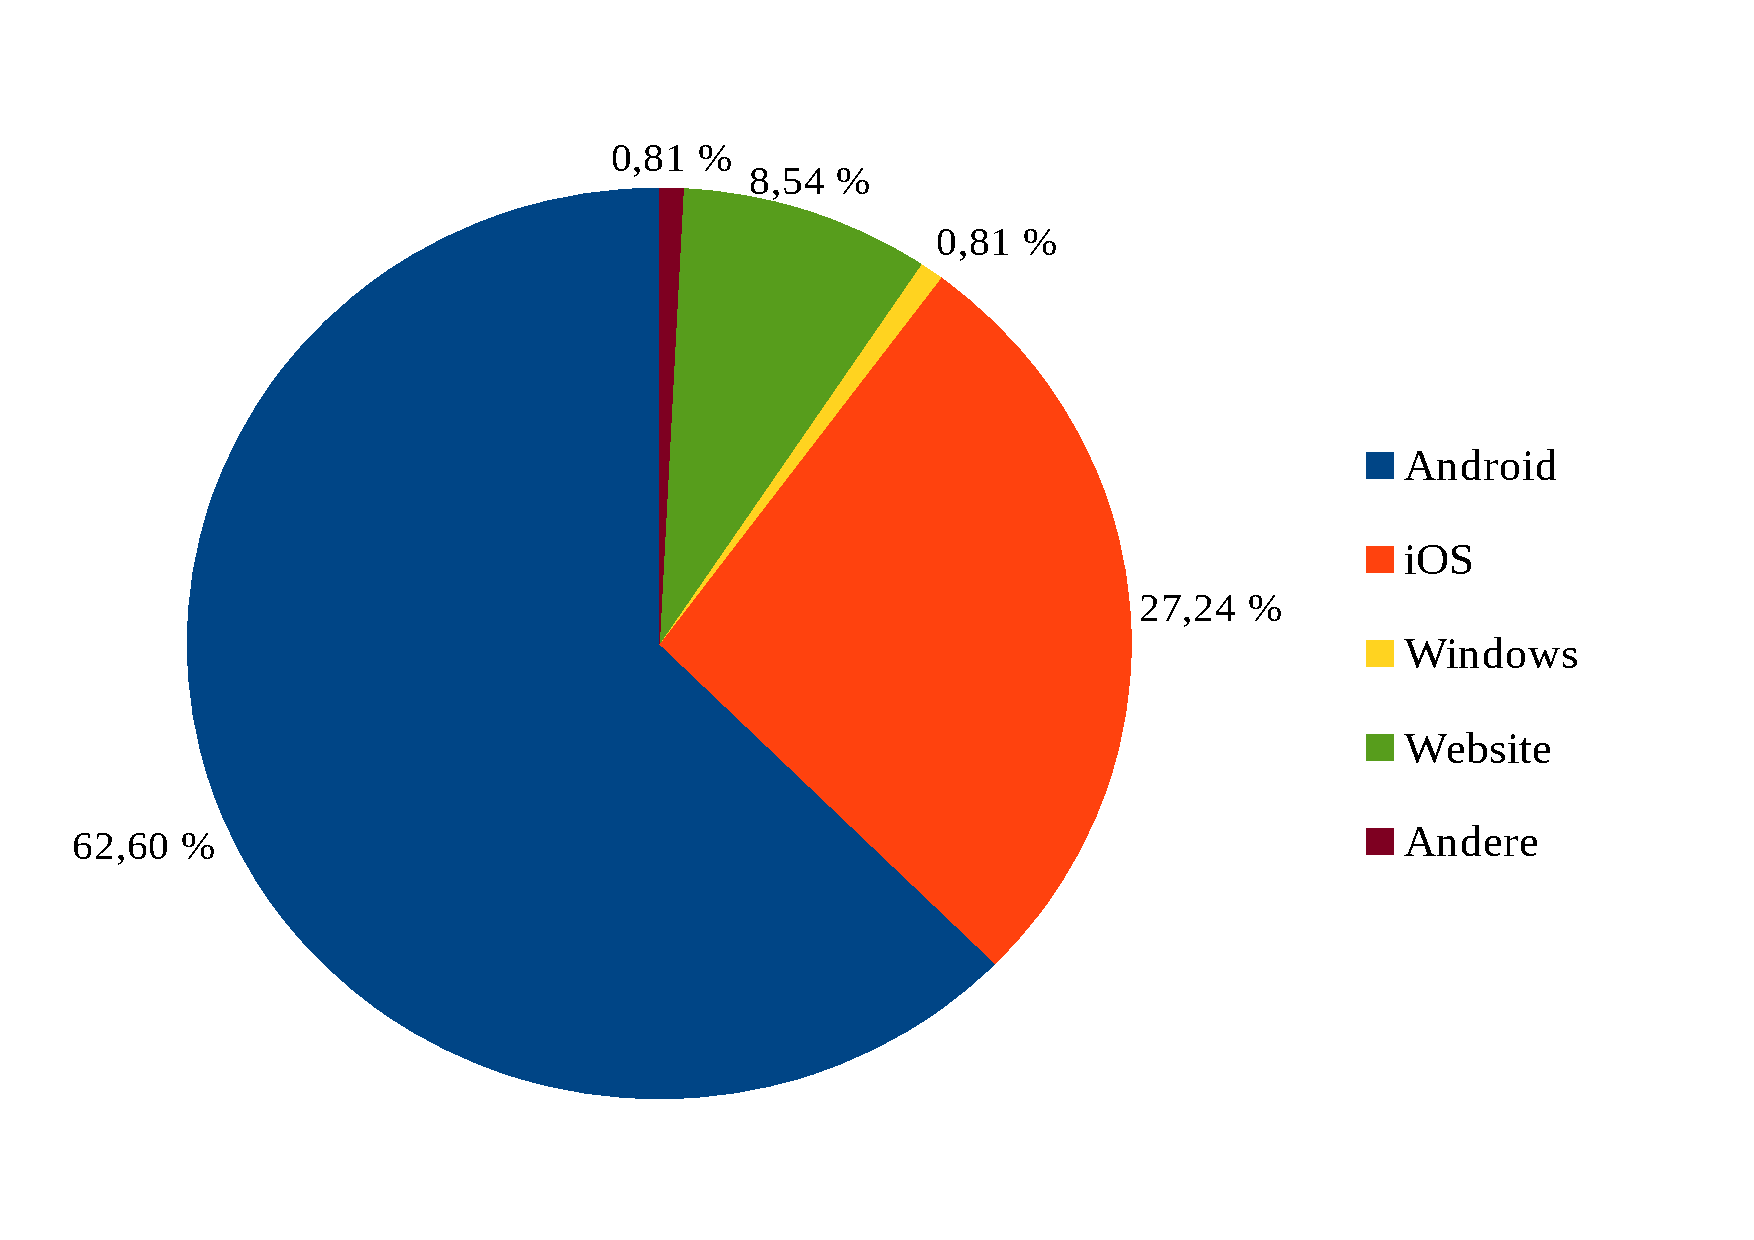
\includegraphics[width=12 cm]{Bilder/Umfrage/Umfrage_Appnutzung.pdf}
		\caption{Umfragewerte zur Nutzung der Apps nach Plattform\label{fig:umfrage_appnutzung}\protect\footnotemark}
	\end{center}
\end{figure}

\footnotetext{Brysiuk, Lehmann (2019)}

Wie man Anhand Abbildung \ref{fig:umfrage_appnutzung} erkennt, wird die Android \ac{App} der Hochschule Hof von 63\% der Studierenden mit Abstand am meisten genutzt, gefolgt von der \ac{iOS}-\ac{App} mit etwa 29\% aller Nutzer. Als letzte große Informationsquelle wird die Hochschul Website von etwa 6\% aller befragten Studierenden genutzt. Die Windows \ac{App} und andere Alternativen werden kaum genutzt. 

\subsection{Android}

Die Android \ac{App} der Hochschule Hof erfreut sich in den vergangenen Jahren großer Beliebtheit bei den Studierenden. Wie bereits gezeigt wurde, ist sie die meist genutzte \ac{App} aller Alternativen aus dem Hochschul Angebot. Neben den Grundfunktionen eines Stundenplans, eines personalisierten Stundenplans und dem Anzeigen der Stundenplanänderungen besitzt die \ac{App} im Vergleich zu den anderen nativen Anwendungen für \ac{iOS} und Windows die meisten zusätzlichen Funktionen. Unter anderem wurde eine Webview des Primuss Portal eingebaut, welche sich nach einem einmaligen Anmelden auch die Anmeldedaten des Nutzers merkt, was mehrfaches Einloggen unnötig macht. Ebenfalls durch eine Webview integriert wurde eine Navigation- und Fahrplanfunktion. Durch diese kann man sich Fahrzeiten und Verbindungen aller öffentlichen Verkehrsmittel anzeigen lassen. Weitere nützliche Funktionen sind die Raumsuche, \textit{Wo bin ich?} und die Chatfunktion für jede Vorlesung.
\\
\linebreak
%Speiseplan
Die Android \ac{App} der Hochschule Hof besitzt ebenfalls eine Schnittstelle, mit der sie Speiseplaninformationen aus dem Angebot des Studentenwerk Oberfrankens anzeigen kann. In dieser kann man seine Vorlieben speichern und sich nur die Speisen anzeigen lassen, welche für den Nutzer selbst relevant sind. Die Funktion ist besonders hervorzuheben, da nicht alle Anwendungen der Hochschule Hof das Menü des Studentenwerks bereitstellen. 

\subsection{iOS}

Mit knapp 29\% der befragten Nutzer liegt die \ac{iOS} Anwendung der Hochschule Hof an zweiter Stelle im Nutzungsranking der Umfrageteilnehmer. Das korreliert auch mit den allgemeinen Marktanteilen der Smartphone Betriebssysteme, welche in Abbildung \ref{fig:smartphoneOS_marktanteile} dargestellt werden\autocite[Vgl.][]{mobileosstatista}. Auch die Grundlegenden Funktionen des Stundenplans sind wie bei der Android \ac{App} vorhanden. Zusätzlich dazu hat der Nutzer die Möglichkeit, die offiziellen Termine der Hochschule Hof einzusehen, sowie eine eigene Aufgabenliste anzulegen und zu pflegen. Als kleinen Zusatz hat die \ac{iOS}-\ac{App} auch ein sogenanntes Widget. Das bedeutet, die Anwendung kann Daten auf dem Bildschirm des Smartphones anzeigen, ohne, dass die \ac{App} geöffnet ist.
\\
\linebreak
Zu bemängeln ist, dass die Nutzer dieser Anwendung keinen direkten Zugriff auf den Speiseplan der Mensa der \ac{HföD AIV} haben. Stattdessen haben befragte Nutzer angegeben, dass sie den Speiseplan über die offizielle Website des Studentenwerk Oberfrankens beziehen, sich aber eine Einbindung in die \ac{App} wünschen\autocite[][]{umfrage}.

\subsection{Windows App}

Die mit Abstand am wenigsten genutzte Anwendung der Hochschule Hof ist die Windows \ac{App}. Nur ein Prozent der befragten Studierenden nutzen demnach diese \ac{App}. Umgerechnet sind das lediglich 2 Nutzer. Trotz der geringen Nutzung bietet die Windows Anwendung ein sauberes Interface, über welches der Nutzer die üblichen Informationen wie die anstehenden Vorlesungen einsehen kann. Auch hier hat der Anwender die Möglichkeit, seinen Stundenplan zu personalisieren. Weitere nützliche Funktionen sucht man hingegen vergeblich. Im Gegensatz zur \ac{iOS}-\ac{App} bietet die Windows \ac{App} dennoch die aktuellen Speiseplan Informationen an.

\subsection{Website}

Als Alternative zur Nutzung der nativen, plattformabhängigen und unabhängig entwickelten Anwendungen der Hochschule Hof soll hier nochmals die Website als Informationsquelle für Stundenplaninformationen und weitere nützliche Daten betrachtet werden. Die Nutzergruppe, die keine der Smartphone \acp{App} nutzt macht immerhin fast 6\% aus und ist damit deutlich größer als die der Windows User.
\\
\linebreak
Stundenplan Informationen können nach einer einfachen Auswahl des Studiengangs und des Fachsemesters eingesehen werden. Weitere Verfeinerungen der Vorlesungen bietet die Art der Veranstaltung, welche die Trefferliste eingrenzt. Zusätzlich bietet die Seite die Möglichkeit an, den Stundenplan als \ac{PDF} herunterzuladen und zu drucken. Ähnlich werden auch die Stundenplanänderungen angezeigt. Nach Auswahl des Studiengangs und des Fachsemesters werden dem Nutzer alle anstehenden Änderungen angezeigt. Zusätzlich kann der Nutzer auch ein Datum angeben, um die Ergebnisse zu filtern.
\\
\linebreak
Um den Mensa Speiseplan des Studentenwerk Oberfrankens mit einzubinden, wurde der Website ein Verweis auf die offizielle Website des Anbieters hinzugefügt. Dieser leitet allerdings nur auf die offizielle Website weiter und bietet keine weiteren Informationen.

\subsection{Fazit}

Im Allgemeinen kann man erkennen, dass die Nutzungsverteilung der \acp{App} der Hochschule Hof mit den Marktanteilen der Smartphone Betriebssysteme in Deutschland korreliert. Dies ist besonders gut in Abbildung \ref{fig:smartphoneOS_marktanteile} zu erkennen\autocite[][]{mobileosstatista}. Da die meisten der Studierenden ein Android betriebenes Handy besitzen, wird diese \ac{App} auch am meisten genutzt. Genauso lässt sich die Nutzung der \ac{iOS}-\ac{App} erklären. 

\begin{figure}[h]
	\begin{center}
		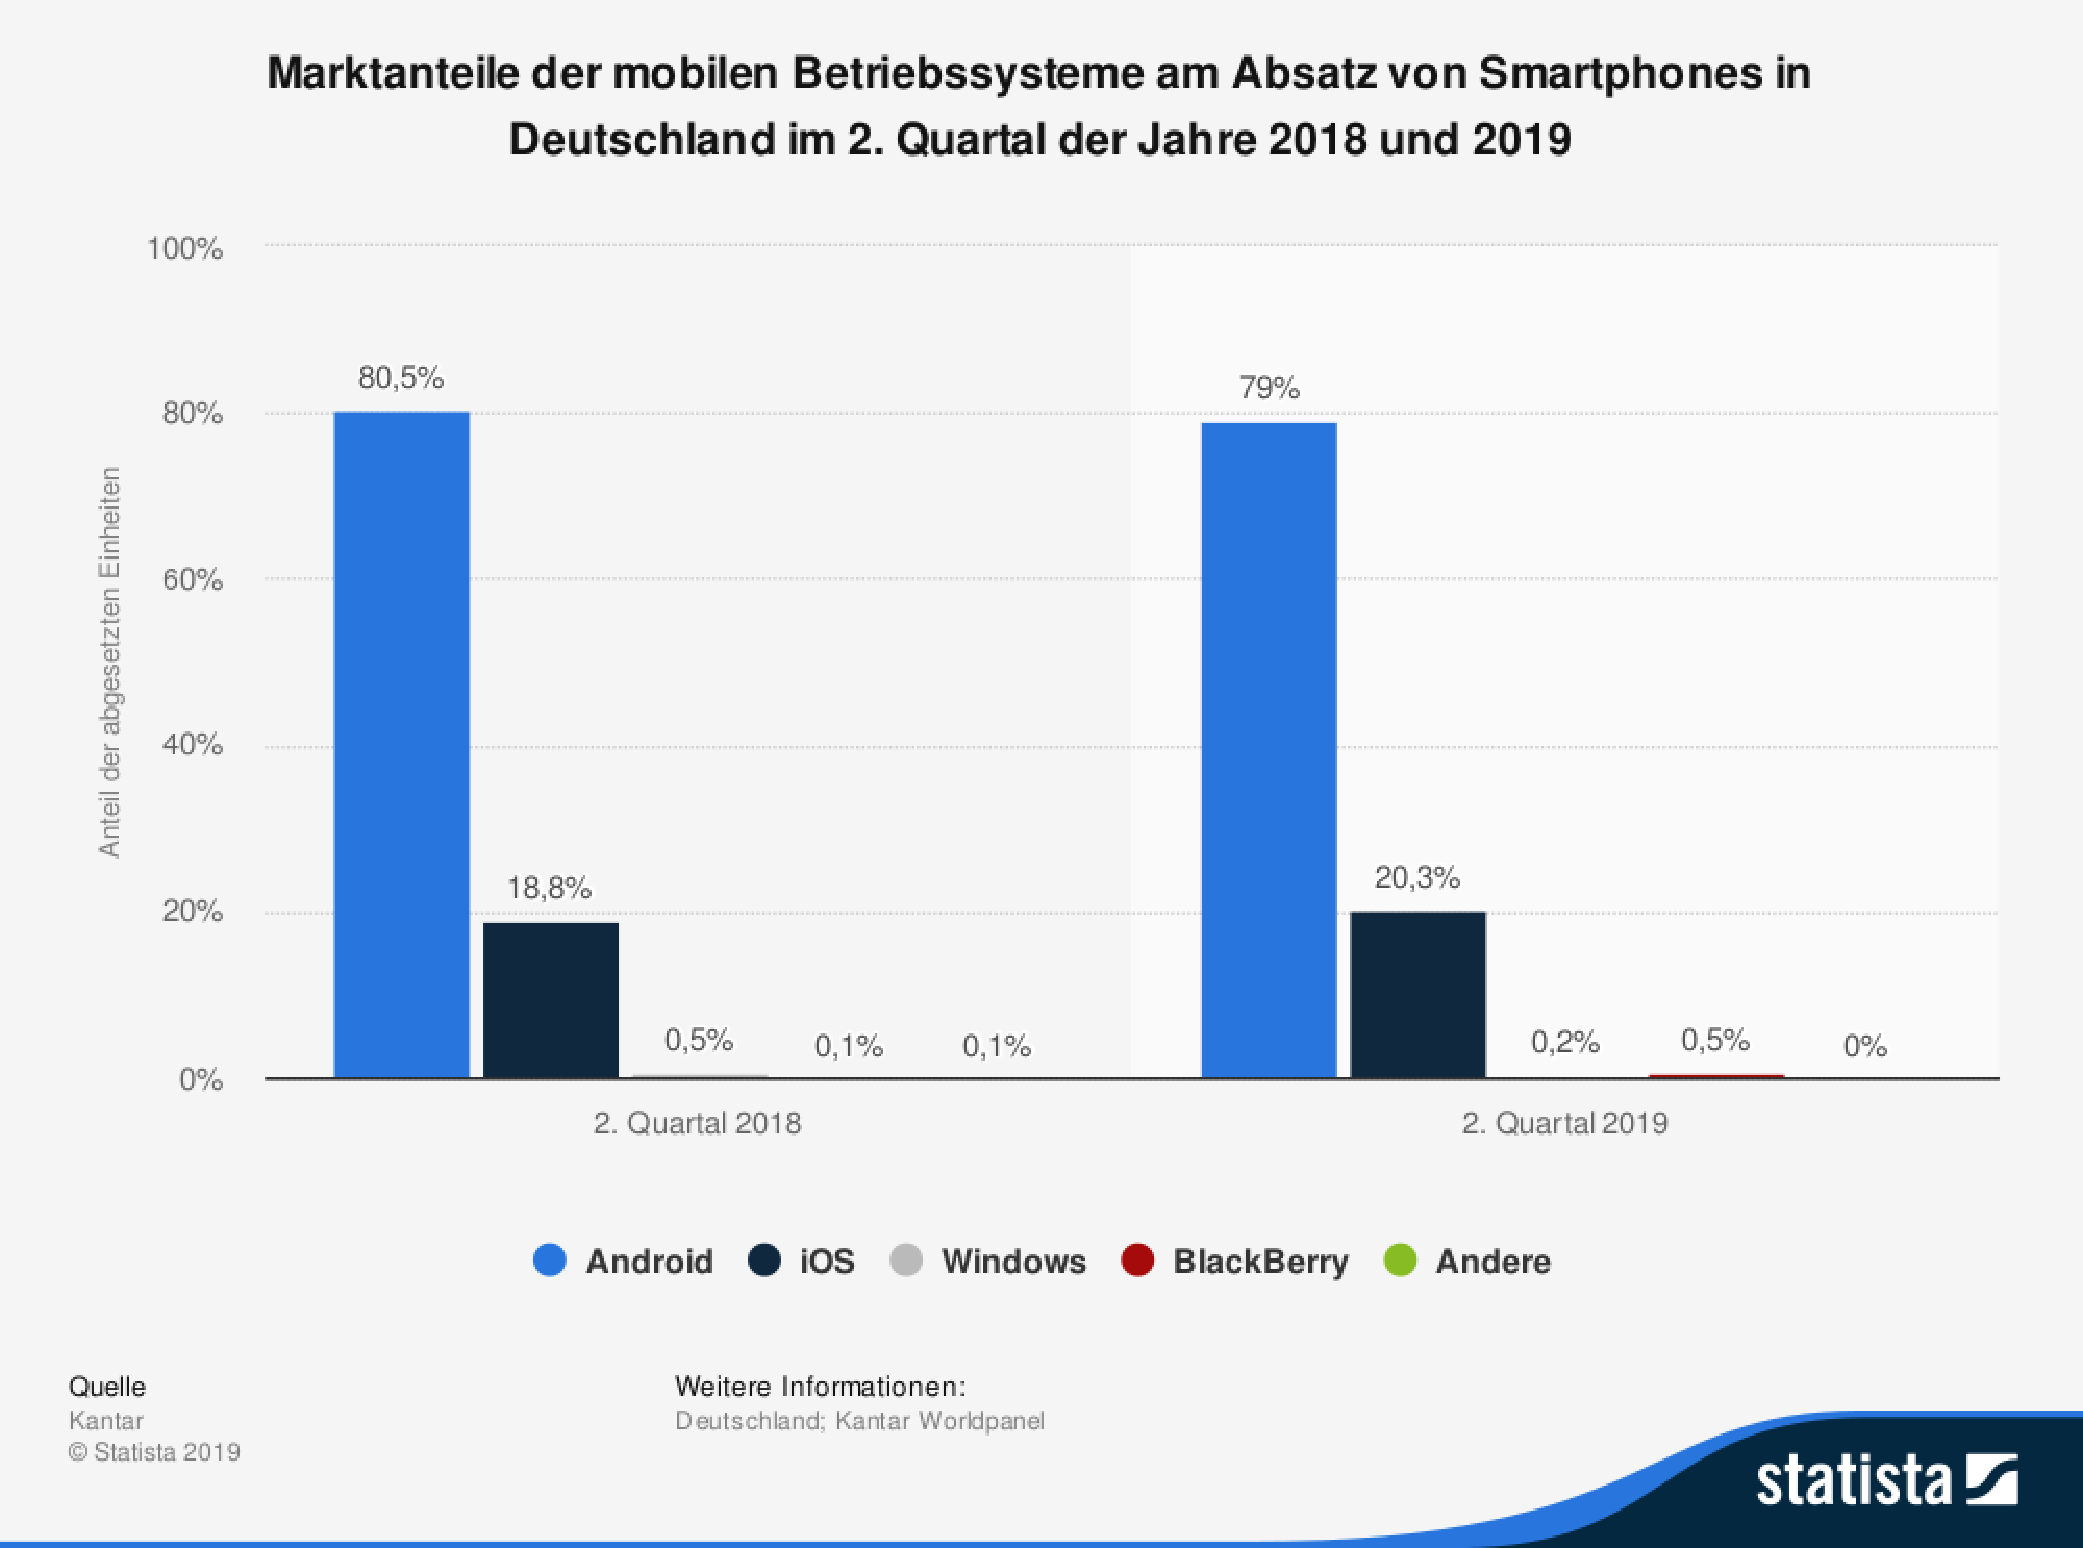
\includegraphics[width=12cm]{Bilder/Statistik/Statista_SmartphoneOS.pdf}
		\caption{Marktanteile der mobilen Betriebssysteme am Absatz von Smartphones in Deutschland im 2. Quartal der Jahre 2018 und 2019\label{fig:smartphoneOS_marktanteile}\protect\footnotemark}
	\end{center}
\end{figure}
\footnotetext{ebd.}

%Kantar. (2019). Marktanteile der mobilen Betriebssysteme am Absatz von Smartphones in Deutschland im 2. Quartal der Jahre 2018 und 2019. Statista. Statista GmbH. Zugriff: 15. August 2019. https://de.statista.com/statistik/daten/studie/198435/umfrage/marktanteile-der-smartphone-betriebssysteme-am-absatz-in-deutschland/

Dennoch ist anzumerken, dass die Android Version die meisten zusätzlichen Features bietet, auch wenn sie laut Nutzerberichten nicht zuverlässig funktionieren und oft auch nicht als sinnvoll eingestuft werden\autocite[Vgl.][]{umfrage}. Auch die Einbindung der Speiseplan-Informationen ist eine gern gesehene Funktion bei den Studierenden und wird demnach auch bei den Nutzern der \ac{iOS}-\ac{App} gefordert.